% GNUPLOT: LaTeX picture with Postscript
\begingroup
  \makeatletter
  \providecommand\color[2][]{%
    \GenericError{(gnuplot) \space\space\space\@spaces}{%
      Package color not loaded in conjunction with
      terminal option `colourtext'%
    }{See the gnuplot documentation for explanation.%
    }{Either use 'blacktext' in gnuplot or load the package
      color.sty in LaTeX.}%
    \renewcommand\color[2][]{}%
  }%
  \providecommand\includegraphics[2][]{%
    \GenericError{(gnuplot) \space\space\space\@spaces}{%
      Package graphicx or graphics not loaded%
    }{See the gnuplot documentation for explanation.%
    }{The gnuplot epslatex terminal needs graphicx.sty or graphics.sty.}%
    \renewcommand\includegraphics[2][]{}%
  }%
  \providecommand\rotatebox[2]{#2}%
  \@ifundefined{ifGPcolor}{%
    \newif\ifGPcolor
    \GPcolortrue
  }{}%
  \@ifundefined{ifGPblacktext}{%
    \newif\ifGPblacktext
    \GPblacktexttrue
  }{}%
  % define a \g@addto@macro without @ in the name:
  \let\gplgaddtomacro\g@addto@macro
  % define empty templates for all commands taking text:
  \gdef\gplbacktext{}%
  \gdef\gplfronttext{}%
  \makeatother
  \ifGPblacktext
    % no textcolor at all
    \def\colorrgb#1{}%
    \def\colorgray#1{}%
  \else
    % gray or color?
    \ifGPcolor
      \def\colorrgb#1{\color[rgb]{#1}}%
      \def\colorgray#1{\color[gray]{#1}}%
      \expandafter\def\csname LTw\endcsname{\color{white}}%
      \expandafter\def\csname LTb\endcsname{\color{black}}%
      \expandafter\def\csname LTa\endcsname{\color{black}}%
      \expandafter\def\csname LT0\endcsname{\color[rgb]{1,0,0}}%
      \expandafter\def\csname LT1\endcsname{\color[rgb]{0,1,0}}%
      \expandafter\def\csname LT2\endcsname{\color[rgb]{0,0,1}}%
      \expandafter\def\csname LT3\endcsname{\color[rgb]{1,0,1}}%
      \expandafter\def\csname LT4\endcsname{\color[rgb]{0,1,1}}%
      \expandafter\def\csname LT5\endcsname{\color[rgb]{1,1,0}}%
      \expandafter\def\csname LT6\endcsname{\color[rgb]{0,0,0}}%
      \expandafter\def\csname LT7\endcsname{\color[rgb]{1,0.3,0}}%
      \expandafter\def\csname LT8\endcsname{\color[rgb]{0.5,0.5,0.5}}%
    \else
      % gray
      \def\colorrgb#1{\color{black}}%
      \def\colorgray#1{\color[gray]{#1}}%
      \expandafter\def\csname LTw\endcsname{\color{white}}%
      \expandafter\def\csname LTb\endcsname{\color{black}}%
      \expandafter\def\csname LTa\endcsname{\color{black}}%
      \expandafter\def\csname LT0\endcsname{\color{black}}%
      \expandafter\def\csname LT1\endcsname{\color{black}}%
      \expandafter\def\csname LT2\endcsname{\color{black}}%
      \expandafter\def\csname LT3\endcsname{\color{black}}%
      \expandafter\def\csname LT4\endcsname{\color{black}}%
      \expandafter\def\csname LT5\endcsname{\color{black}}%
      \expandafter\def\csname LT6\endcsname{\color{black}}%
      \expandafter\def\csname LT7\endcsname{\color{black}}%
      \expandafter\def\csname LT8\endcsname{\color{black}}%
    \fi
  \fi
    \setlength{\unitlength}{0.0500bp}%
    \ifx\gptboxheight\undefined%
      \newlength{\gptboxheight}%
      \newlength{\gptboxwidth}%
      \newsavebox{\gptboxtext}%
    \fi%
    \setlength{\fboxrule}{0.5pt}%
    \setlength{\fboxsep}{1pt}%
\begin{picture}(9620.00,9620.00)%
    \gplgaddtomacro\gplbacktext{%
      \csname LTb\endcsname%
      \put(867,5057){\makebox(0,0)[r]{\strut{}$15000$}}%
      \csname LTb\endcsname%
      \put(867,5470){\makebox(0,0)[r]{\strut{}$20000$}}%
      \csname LTb\endcsname%
      \put(867,5883){\makebox(0,0)[r]{\strut{}$25000$}}%
      \csname LTb\endcsname%
      \put(867,6296){\makebox(0,0)[r]{\strut{}$30000$}}%
      \csname LTb\endcsname%
      \put(867,6709){\makebox(0,0)[r]{\strut{}$35000$}}%
      \csname LTb\endcsname%
      \put(867,7123){\makebox(0,0)[r]{\strut{}$40000$}}%
      \csname LTb\endcsname%
      \put(867,7536){\makebox(0,0)[r]{\strut{}$45000$}}%
      \csname LTb\endcsname%
      \put(867,7949){\makebox(0,0)[r]{\strut{}$50000$}}%
      \csname LTb\endcsname%
      \put(867,8362){\makebox(0,0)[r]{\strut{}$55000$}}%
      \csname LTb\endcsname%
      \put(867,8775){\makebox(0,0)[r]{\strut{}$60000$}}%
      \csname LTb\endcsname%
      \put(955,4858){\makebox(0,0){\strut{}$2^{1}$}}%
      \csname LTb\endcsname%
      \put(1579,4858){\makebox(0,0){\strut{}$2^{2}$}}%
      \csname LTb\endcsname%
      \put(2203,4858){\makebox(0,0){\strut{}$2^{3}$}}%
      \csname LTb\endcsname%
      \put(2827,4858){\makebox(0,0){\strut{}$2^{4}$}}%
      \csname LTb\endcsname%
      \put(3451,4858){\makebox(0,0){\strut{}$2^{5}$}}%
      \csname LTb\endcsname%
      \put(4075,4858){\makebox(0,0){\strut{}$2^{6}$}}%
      \csname LTb\endcsname%
      \put(4163,5057){\makebox(0,0)[l]{\strut{} }}%
      \csname LTb\endcsname%
      \put(4163,5470){\makebox(0,0)[l]{\strut{} }}%
      \csname LTb\endcsname%
      \put(4163,5883){\makebox(0,0)[l]{\strut{} }}%
      \csname LTb\endcsname%
      \put(4163,6296){\makebox(0,0)[l]{\strut{} }}%
      \csname LTb\endcsname%
      \put(4163,6709){\makebox(0,0)[l]{\strut{} }}%
      \csname LTb\endcsname%
      \put(4163,7123){\makebox(0,0)[l]{\strut{} }}%
      \csname LTb\endcsname%
      \put(4163,7536){\makebox(0,0)[l]{\strut{} }}%
      \csname LTb\endcsname%
      \put(4163,7949){\makebox(0,0)[l]{\strut{} }}%
      \csname LTb\endcsname%
      \put(4163,8362){\makebox(0,0)[l]{\strut{} }}%
      \csname LTb\endcsname%
      \put(4163,8775){\makebox(0,0)[l]{\strut{} }}%
      \csname LTb\endcsname%
      \put(955,8974){\makebox(0,0){\strut{} }}%
      \csname LTb\endcsname%
      \put(1579,8974){\makebox(0,0){\strut{} }}%
      \csname LTb\endcsname%
      \put(2203,8974){\makebox(0,0){\strut{} }}%
      \csname LTb\endcsname%
      \put(2827,8974){\makebox(0,0){\strut{} }}%
      \csname LTb\endcsname%
      \put(3451,8974){\makebox(0,0){\strut{} }}%
      \csname LTb\endcsname%
      \put(4075,8974){\makebox(0,0){\strut{} }}%
    }%
    \gplgaddtomacro\gplfronttext{%
      \csname LTb\endcsname%
      \put(239,6916){\rotatebox{-270}{\makebox(0,0){\strut{}Time [s]}}}%
      \csname LTb\endcsname%
      \put(8827,8675){\makebox(0,0)[r]{\strut{}Picard SoftGMRES Swz w Coarse MGLevels3}}%
      \csname LTb\endcsname%
      \put(8827,8476){\makebox(0,0)[r]{\strut{}NewtonGmres Automatic MGLevels3}}%
      \csname LTb\endcsname%
      \put(8827,8277){\makebox(0,0)[r]{\strut{}NewtonGmres Swz w Coarse Overlap MGLevels3}}%
      \csname LTb\endcsname%
      \put(8827,8078){\makebox(0,0)[r]{\strut{}NewtonGmres Swz w Coarse MGLevels2}}%
      \csname LTb\endcsname%
      \put(8827,7879){\makebox(0,0)[r]{\strut{}NewtonGmres Swz Kcycle w Coarse Overlap MGLevels3}}%
    }%
    \gplgaddtomacro\gplbacktext{%
      \csname LTb\endcsname%
      \put(603,684){\makebox(0,0)[r]{\strut{}$2^{1}$}}%
      \csname LTb\endcsname%
      \put(603,1460){\makebox(0,0)[r]{\strut{}$2^{2}$}}%
      \csname LTb\endcsname%
      \put(603,2235){\makebox(0,0)[r]{\strut{}$2^{3}$}}%
      \csname LTb\endcsname%
      \put(603,3011){\makebox(0,0)[r]{\strut{}$2^{4}$}}%
      \csname LTb\endcsname%
      \put(603,3786){\makebox(0,0)[r]{\strut{}$2^{5}$}}%
      \csname LTb\endcsname%
      \put(603,4562){\makebox(0,0)[r]{\strut{}$2^{6}$}}%
      \csname LTb\endcsname%
      \put(691,485){\makebox(0,0){\strut{}$2^{1}$}}%
      \csname LTb\endcsname%
      \put(1368,485){\makebox(0,0){\strut{}$2^{2}$}}%
      \csname LTb\endcsname%
      \put(2045,485){\makebox(0,0){\strut{}$2^{3}$}}%
      \csname LTb\endcsname%
      \put(2721,485){\makebox(0,0){\strut{}$2^{4}$}}%
      \csname LTb\endcsname%
      \put(3398,485){\makebox(0,0){\strut{}$2^{5}$}}%
      \csname LTb\endcsname%
      \put(4075,485){\makebox(0,0){\strut{}$2^{6}$}}%
      \csname LTb\endcsname%
      \put(4163,684){\makebox(0,0)[l]{\strut{} }}%
      \csname LTb\endcsname%
      \put(4163,1460){\makebox(0,0)[l]{\strut{} }}%
      \csname LTb\endcsname%
      \put(4163,2235){\makebox(0,0)[l]{\strut{} }}%
      \csname LTb\endcsname%
      \put(4163,3011){\makebox(0,0)[l]{\strut{} }}%
      \csname LTb\endcsname%
      \put(4163,3786){\makebox(0,0)[l]{\strut{} }}%
      \csname LTb\endcsname%
      \put(4163,4562){\makebox(0,0)[l]{\strut{} }}%
      \csname LTb\endcsname%
      \put(691,4761){\makebox(0,0){\strut{} }}%
      \csname LTb\endcsname%
      \put(1368,4761){\makebox(0,0){\strut{} }}%
      \csname LTb\endcsname%
      \put(2045,4761){\makebox(0,0){\strut{} }}%
      \csname LTb\endcsname%
      \put(2721,4761){\makebox(0,0){\strut{} }}%
      \csname LTb\endcsname%
      \put(3398,4761){\makebox(0,0){\strut{} }}%
      \csname LTb\endcsname%
      \put(4075,4761){\makebox(0,0){\strut{} }}%
    }%
    \gplgaddtomacro\gplfronttext{%
      \csname LTb\endcsname%
      \put(239,2623){\rotatebox{-270}{\makebox(0,0){\strut{}Speedup}}}%
      \csname LTb\endcsname%
      \put(2383,187){\makebox(0,0){\strut{}Processors}}%
      \csname LTb\endcsname%
      \put(8827,4462){\makebox(0,0)[r]{\strut{}Picard SoftGMRES Swz w Coarse MGLevels3}}%
      \csname LTb\endcsname%
      \put(8827,4263){\makebox(0,0)[r]{\strut{}NewtonGmres Automatic MGLevels3}}%
      \csname LTb\endcsname%
      \put(8827,4064){\makebox(0,0)[r]{\strut{}NewtonGmres Swz w Coarse Overlap MGLevels3}}%
      \csname LTb\endcsname%
      \put(8827,3865){\makebox(0,0)[r]{\strut{}NewtonGmres Swz w Coarse MGLevels2}}%
      \csname LTb\endcsname%
      \put(8827,3666){\makebox(0,0)[r]{\strut{}NewtonGmres Swz Kcycle w Coarse Overlap MGLevels3}}%
      \csname LTb\endcsname%
      \put(8827,3467){\makebox(0,0)[r]{\strut{}Ideal}}%
    }%
    \gplbacktext
    \put(0,0){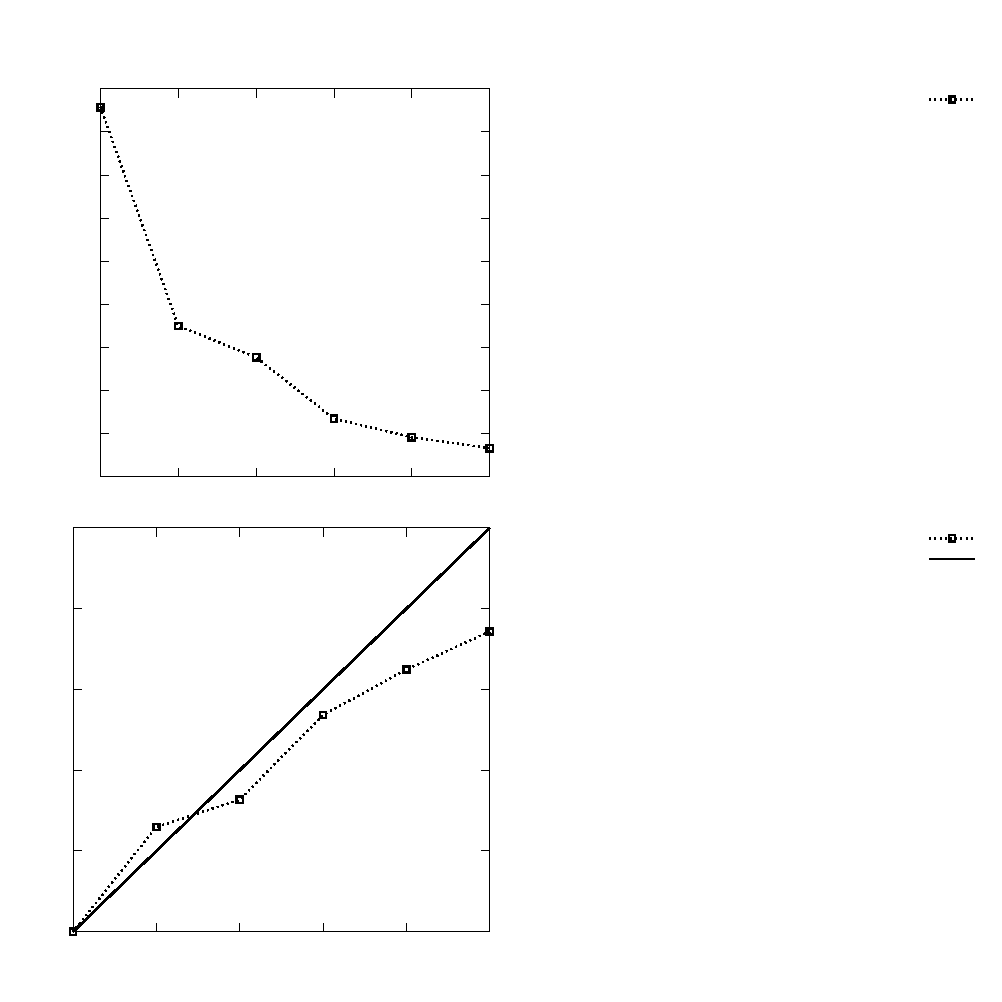
\includegraphics{MPIScalingTimes}}%
    \gplfronttext
  \end{picture}%
\endgroup
